\documentclass[a4paper,10pt]{scrartcl}

\usepackage[utf8]{inputenc}
\usepackage[ngerman]{babel}
\usepackage[T1]{fontenc}
\usepackage{amsmath}
\usepackage{graphicx}
\usepackage{hyperref}
\usepackage{eso-pic} 
\usepackage{mathtools}

\newcommand\BackgroundPic{% 
   \put(0,0){% 
      \parbox[b][\paperheight]{\paperwidth}{% 
         \vfill 
         \centering{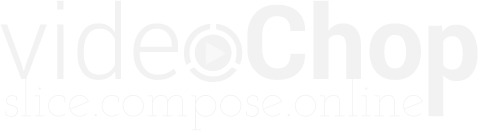
\includegraphics{images/videoChop.png}} 
         \vfill 
      } 
   } 
} 

\title{Medienprojekt I \\ Thema: Videochop}
\author{Michael Duve, Felix Maulwurf, Angelina Staeck}
\date{29.11.2014}
\begin{document}
\maketitle
\newpage
\AddToShipoutPicture{\BackgroundPic}
\tableofcontents
\newpage
\section{Projektteilnehmer}
\subsection{Michael Duve}
\begin{center}

\includegraphics[height=90px, width=90px]{images/micha.jpg}\\
\textbf{Medieninformatik Fachsemester 4} \\
\vspace*{1.5mm} 
HTML5, CSS3, JS, PHP, MySQL, Webapps iOS,\\
Grundkenntnisse Server,
Java, min. Python
Photoshop, Illustrator, InDesign
Repositories (Git, Mercurial), JIRA, Documentation
\end{center}
\subsection{Felix Maulwurf}
\begin{center}

\includegraphics[height=90px, width=90px]{images/felix.jpg}\\
\textbf{Medieninformatik Fachsemester 4} \\
\vspace*{1.5mm} 
HTML5, CSS3, JS, PHP, MySQL, Java,\\
Photoshop, Illustrator, After Effects,
3DSMax,\\
Cinema4D, Office, Repositories (Git), LaTeX
\end{center}
\subsection{Angelina Staeck}
\begin{center}

\includegraphics[height=90px, width=90px]{images/angi.jpg}\\
\textbf{Medieninformatik Fachsemester 4} \\
\vspace*{1.5mm} 
HTML5, CSS3, JS, PHP, \\
Java, SQL, Illustrator, Photoshop
\end{center}
\newpage
\section{Projektbeschreibung}
VideoChop ist eine Webanwendung basierend auf JavaScript, die dem Anwender  ein einfaches und intuitives „Videoschnittstudio“ zur Verfügung stellt. VideoChop soll es ermöglichen Videos vom Desktop direkt in den Browser zu ziehen. Es steht dem User frei, ob er ein oder mehrere Videos schneiden oder zusammenfügen möchte. VideoChop wird eine übersichtliche und schlichte Oberfläche bieten, die auch Anfänger nicht überfordert. Die Videos werden in einer Zeitleiste organisiert und beschnitten. Wer mal eben schnell ein Video schneiden will, um Vor- oder Abspann oder etwaige Längen zu entfernen, braucht keine Speicher fressende und kompliziert zu bedienende Videobearbeitung. Der Nutzer kann sich sein Werk vor dem Abspeichern im Browser als Vorschau ansehen.
\subsection{Idee}
Die Idee ist es, dass VideoChop dem Nutzer eine Plattform zur Verfügung stellt, die keinerlei Daten serverbasiert speichert. Das Projekt basiert auf JavaScript und nutzt somit die Rechenressourcen des Nutzers. Die Belastung für den Server sind damit minimal. VideoChop soll einfach, intuitiv und schnell sein. JavaScript ist sehr mächtig, allerdings sind zu Projektbeginn die Möglichkeiten und Umsetzbarkeiten noch nicht geklärt.
\subsection{Zukunft}
Zukünftig sollen weitere Funktionalitäten hinzukommen. 
\subsection{Probleme}
Das Verbinden mehrerer Videos zu einem mit Hilfe von JavaScript ist sehr problematisch.
\newpage
\section{Mockup}
\textbf{mockup - mockup-vc-MD.pdf} \\
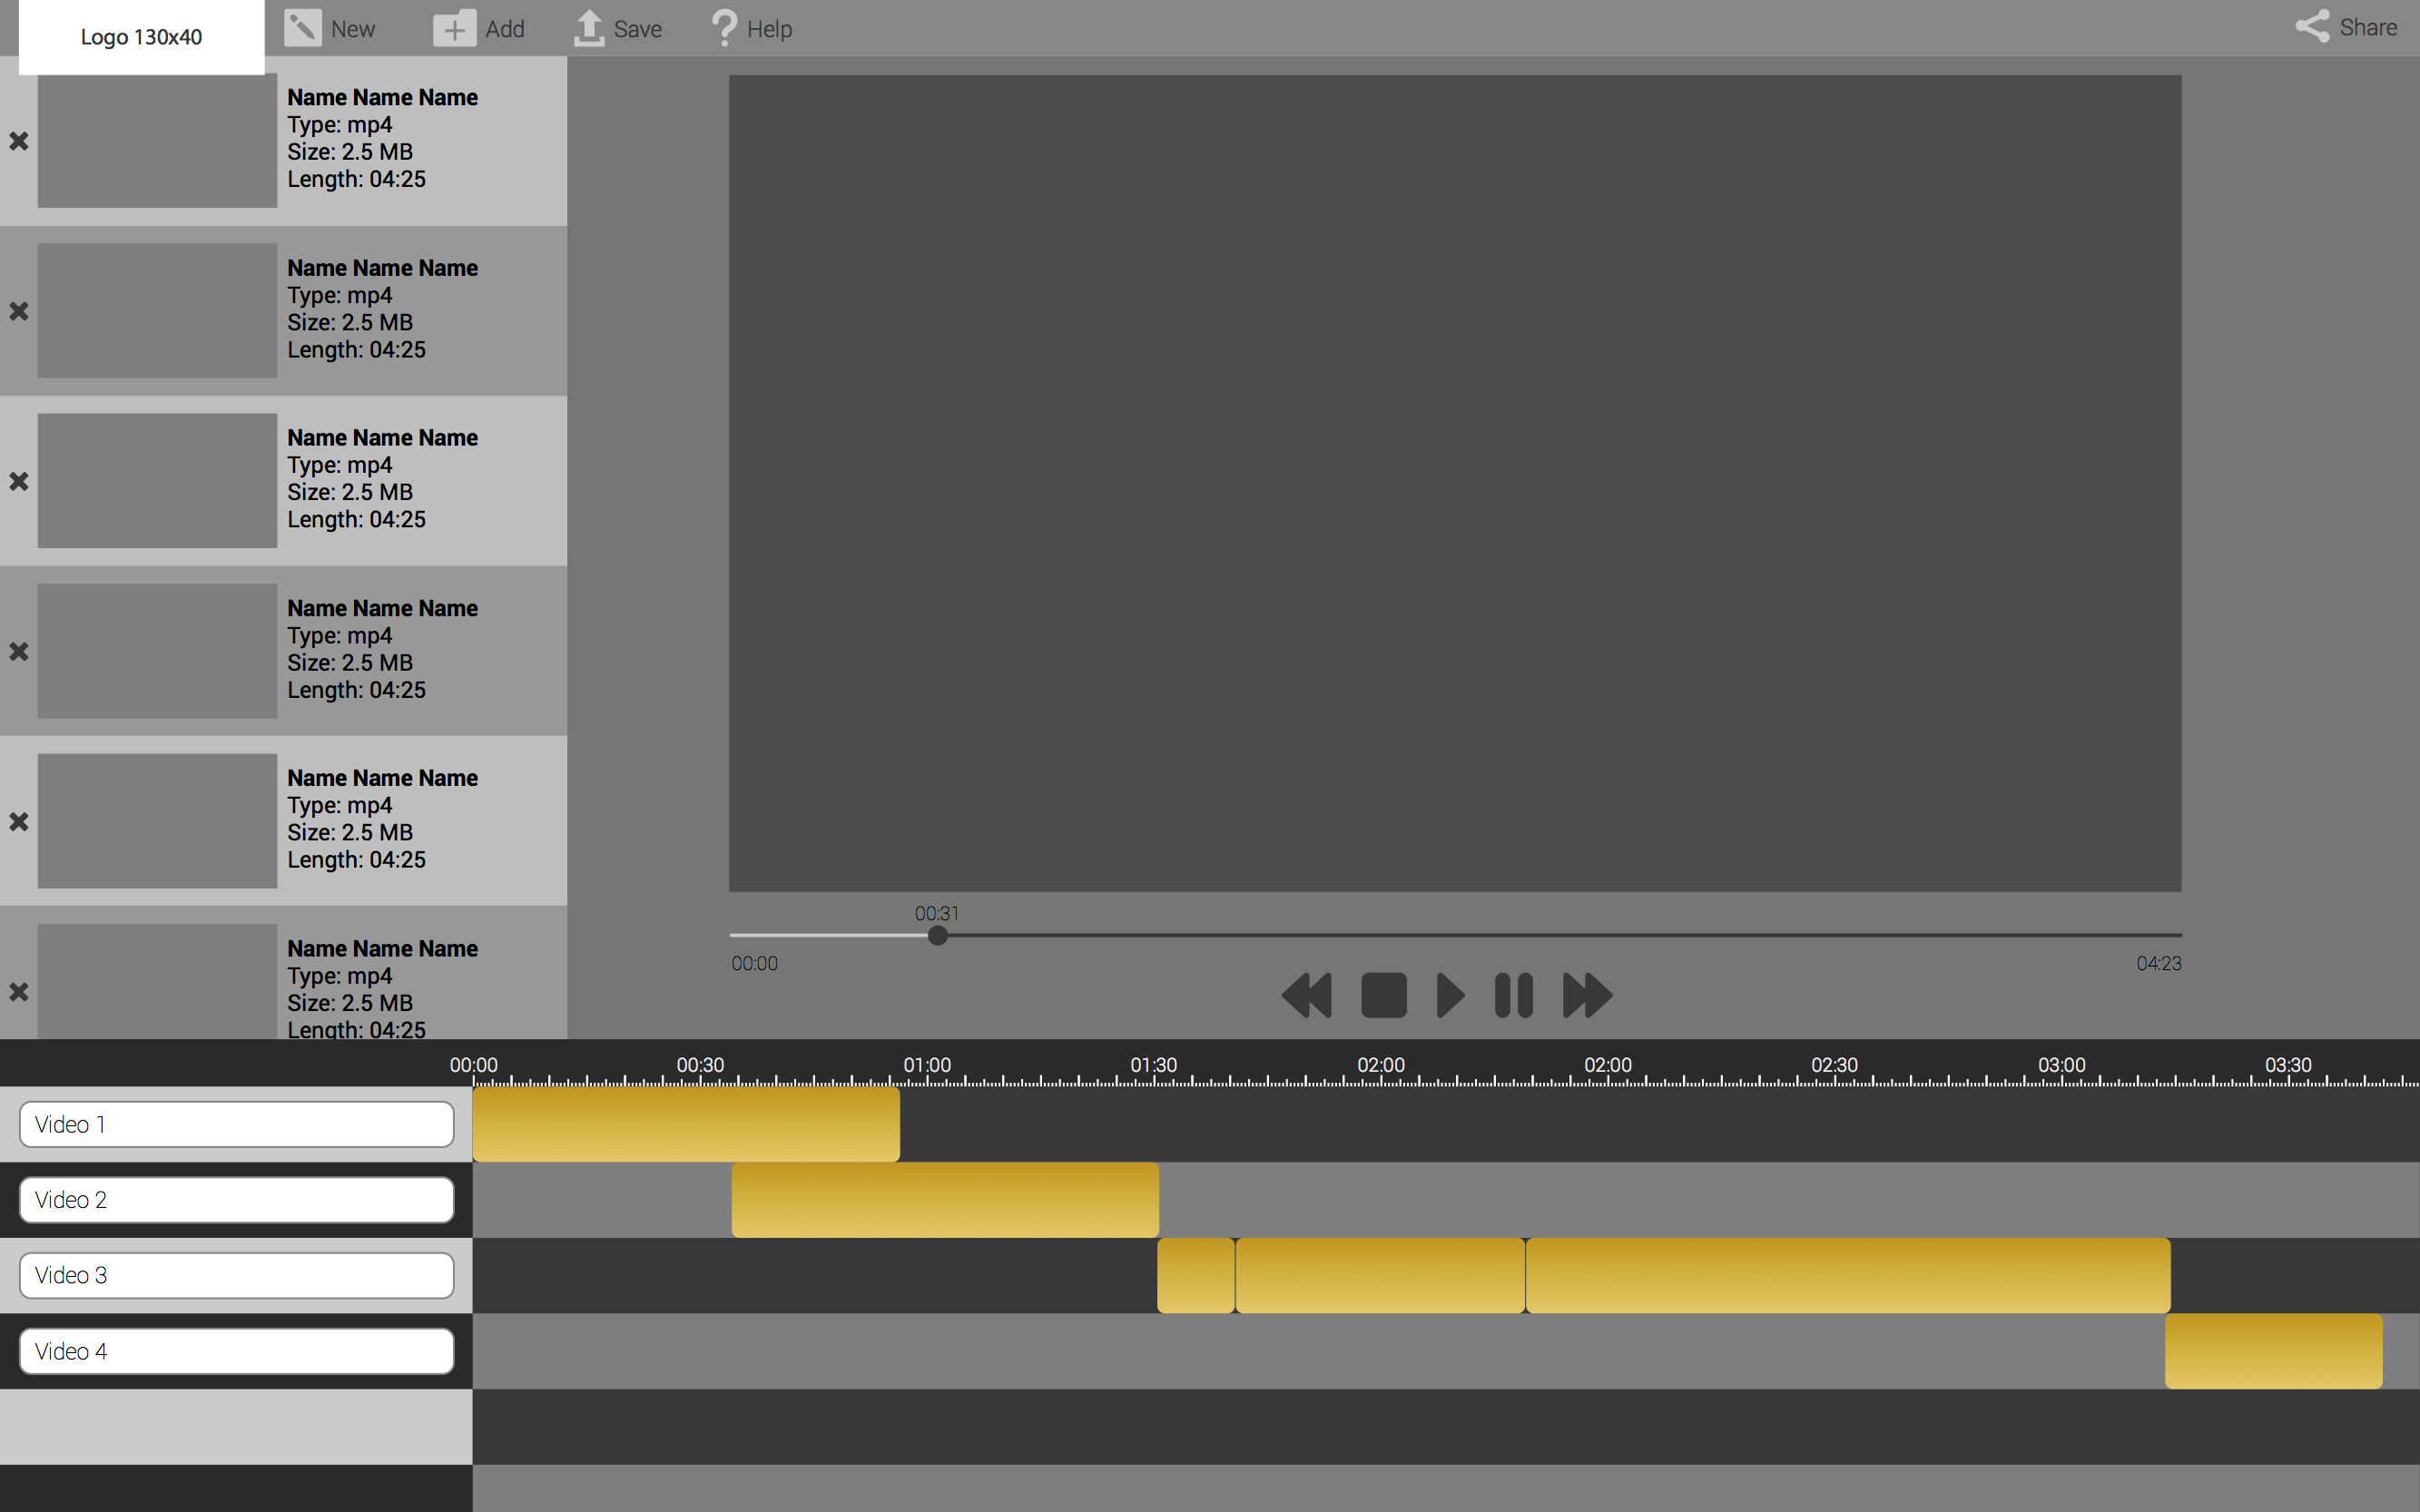
\includegraphics[height=225px, width=390px]{images/mockup.png}\\
\vspace*{1mm}
Das Mockup ist nur eine Orientierung für die finale Website.\\ 
\textbf{mockup - mockup-vc-md-Ideen-und-Kommentare.pdf} \\
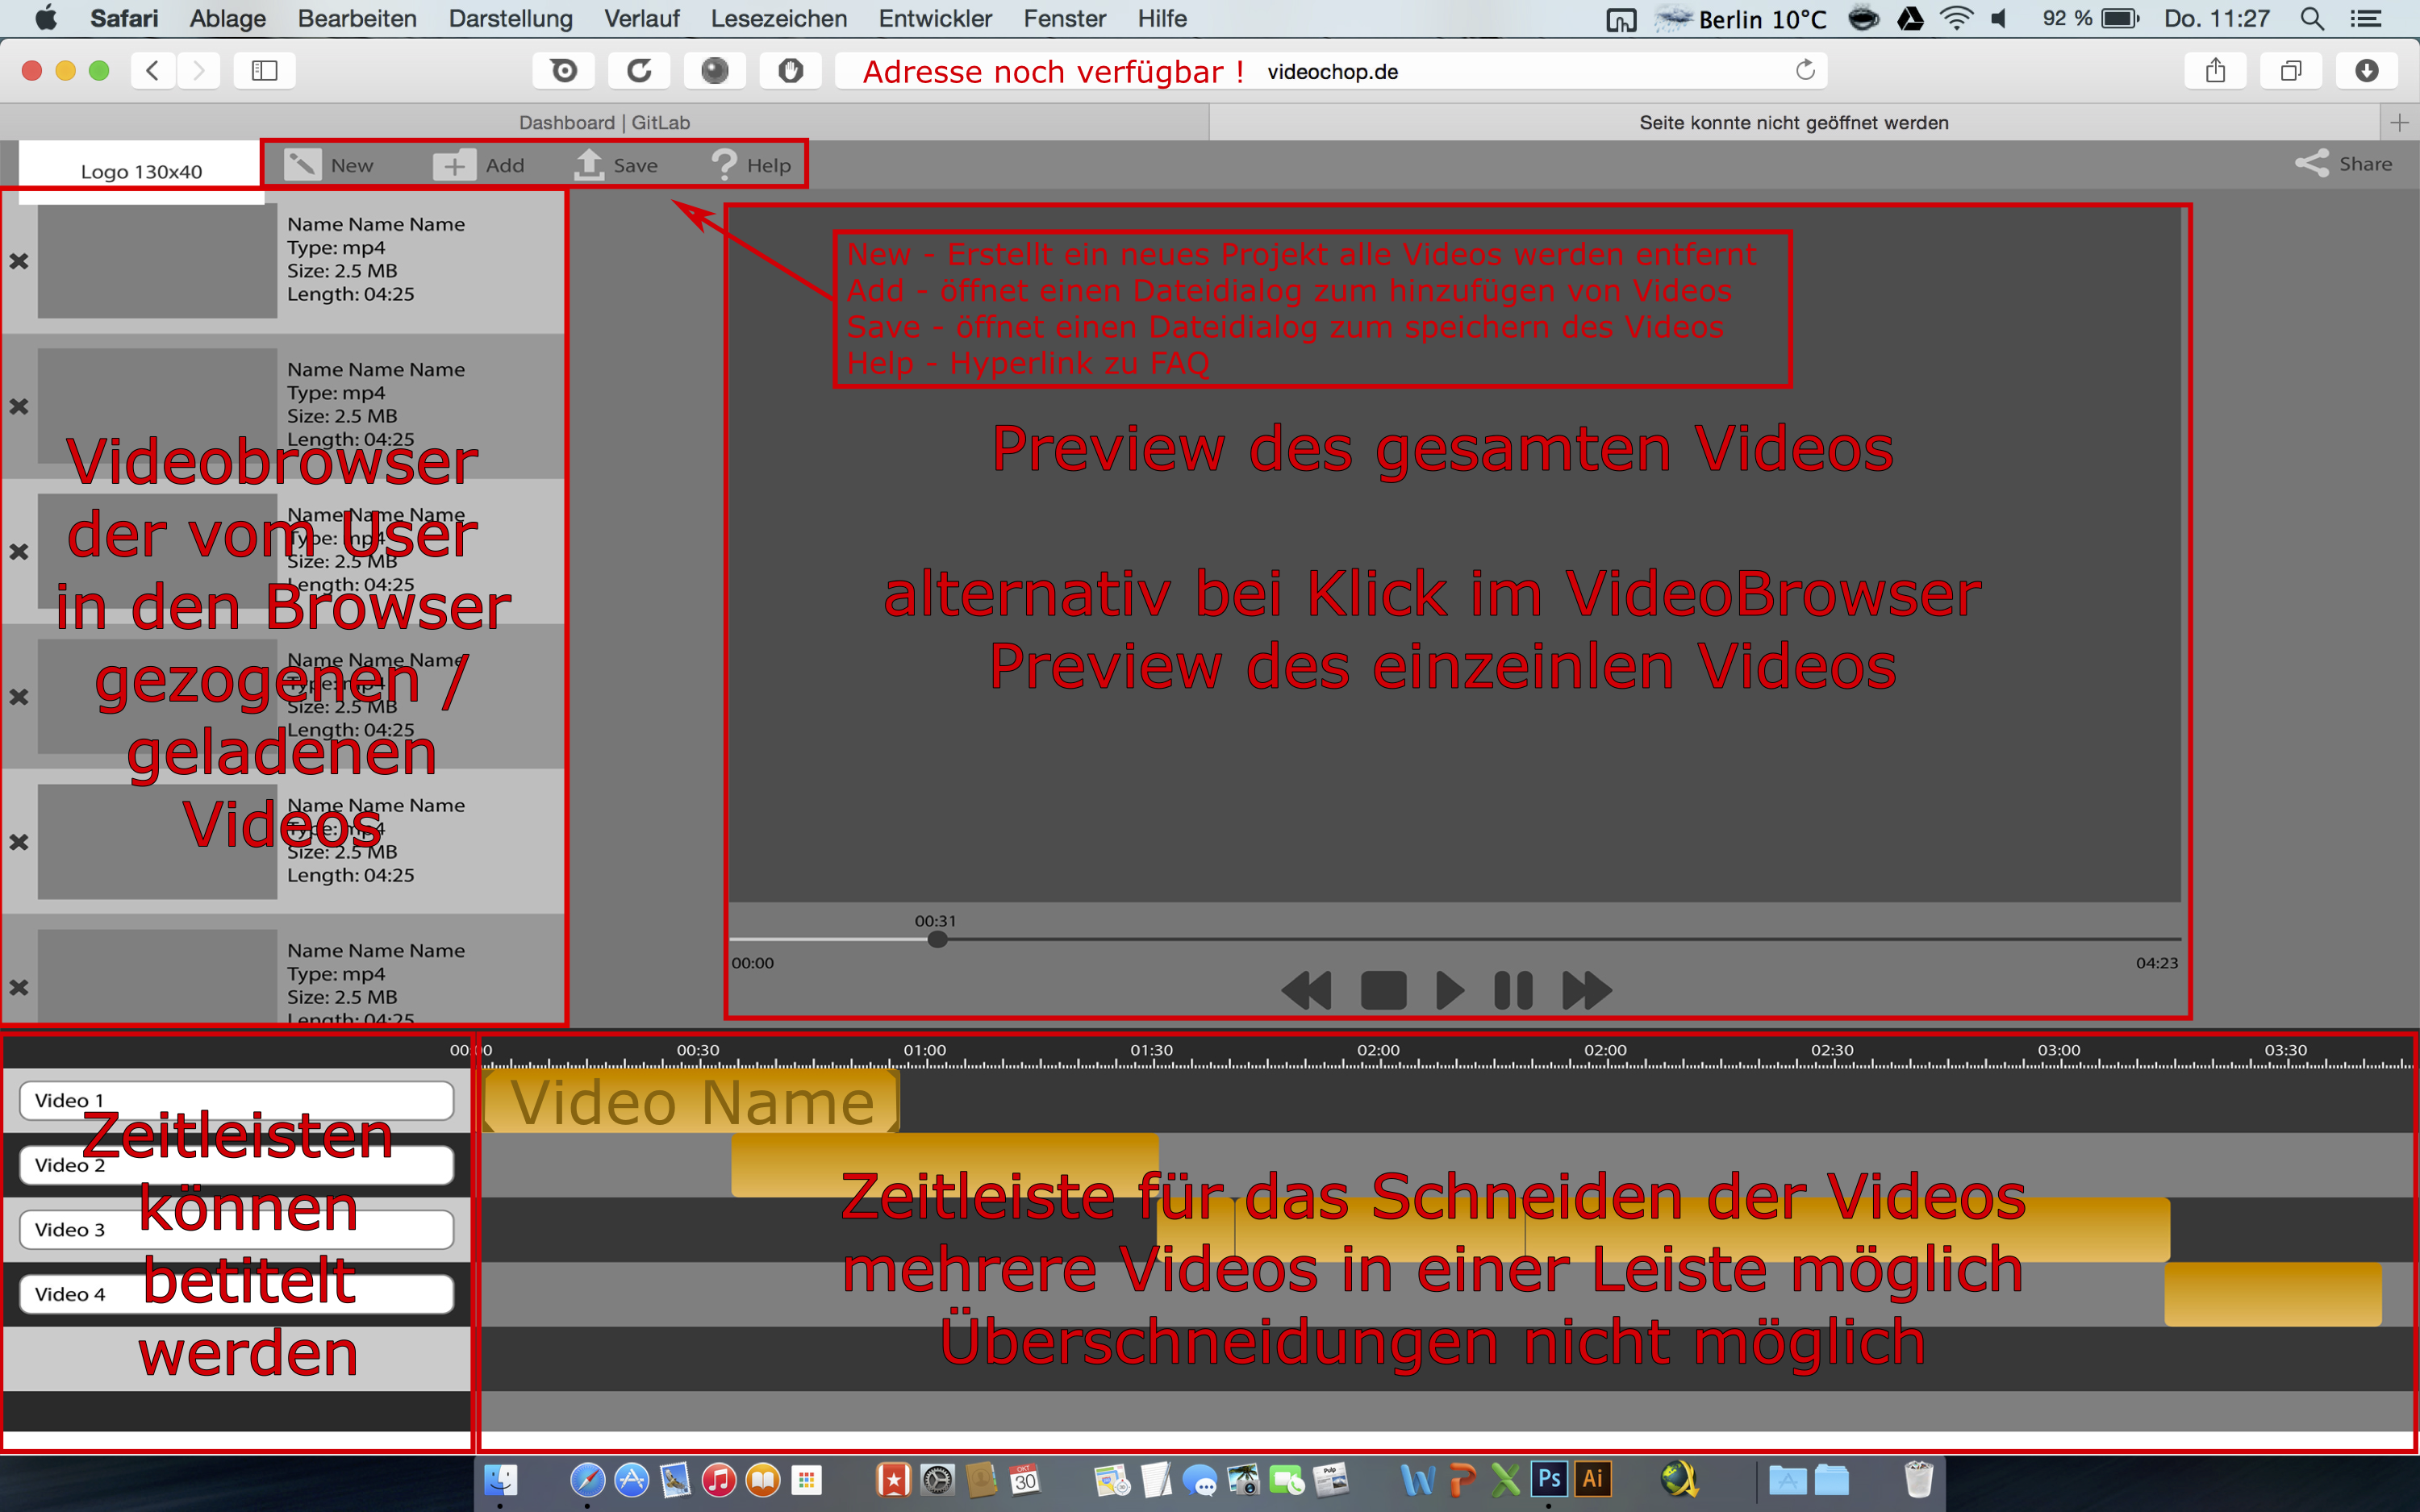
\includegraphics[height=225px, width=390px]{images/mockup2.png}\\
Es wurde in Gruppenarbeit erstellt.
\newpage
\section{Testcases}
Für jede Funktion haben wir Testcases erstellt. Die Testcases werden jeweils nach Bedarf erweitert. Das bedeutet, dass im weiteren Verlauf der Entwicklung neue Testcases hinzukommen können. Die Testcases sind spezifisch und nicht modular programmiert. Aus den Testcases haben wir unsere Module abgeleitet.
\subsection{Canvas}
\textbf{testcases - canvas - index.html} \\
Allgemeiner Funtkionstest des Canvas Objekts.\\ 
\includegraphics[height=176px, width=300px]{images/canvas1.png}\\
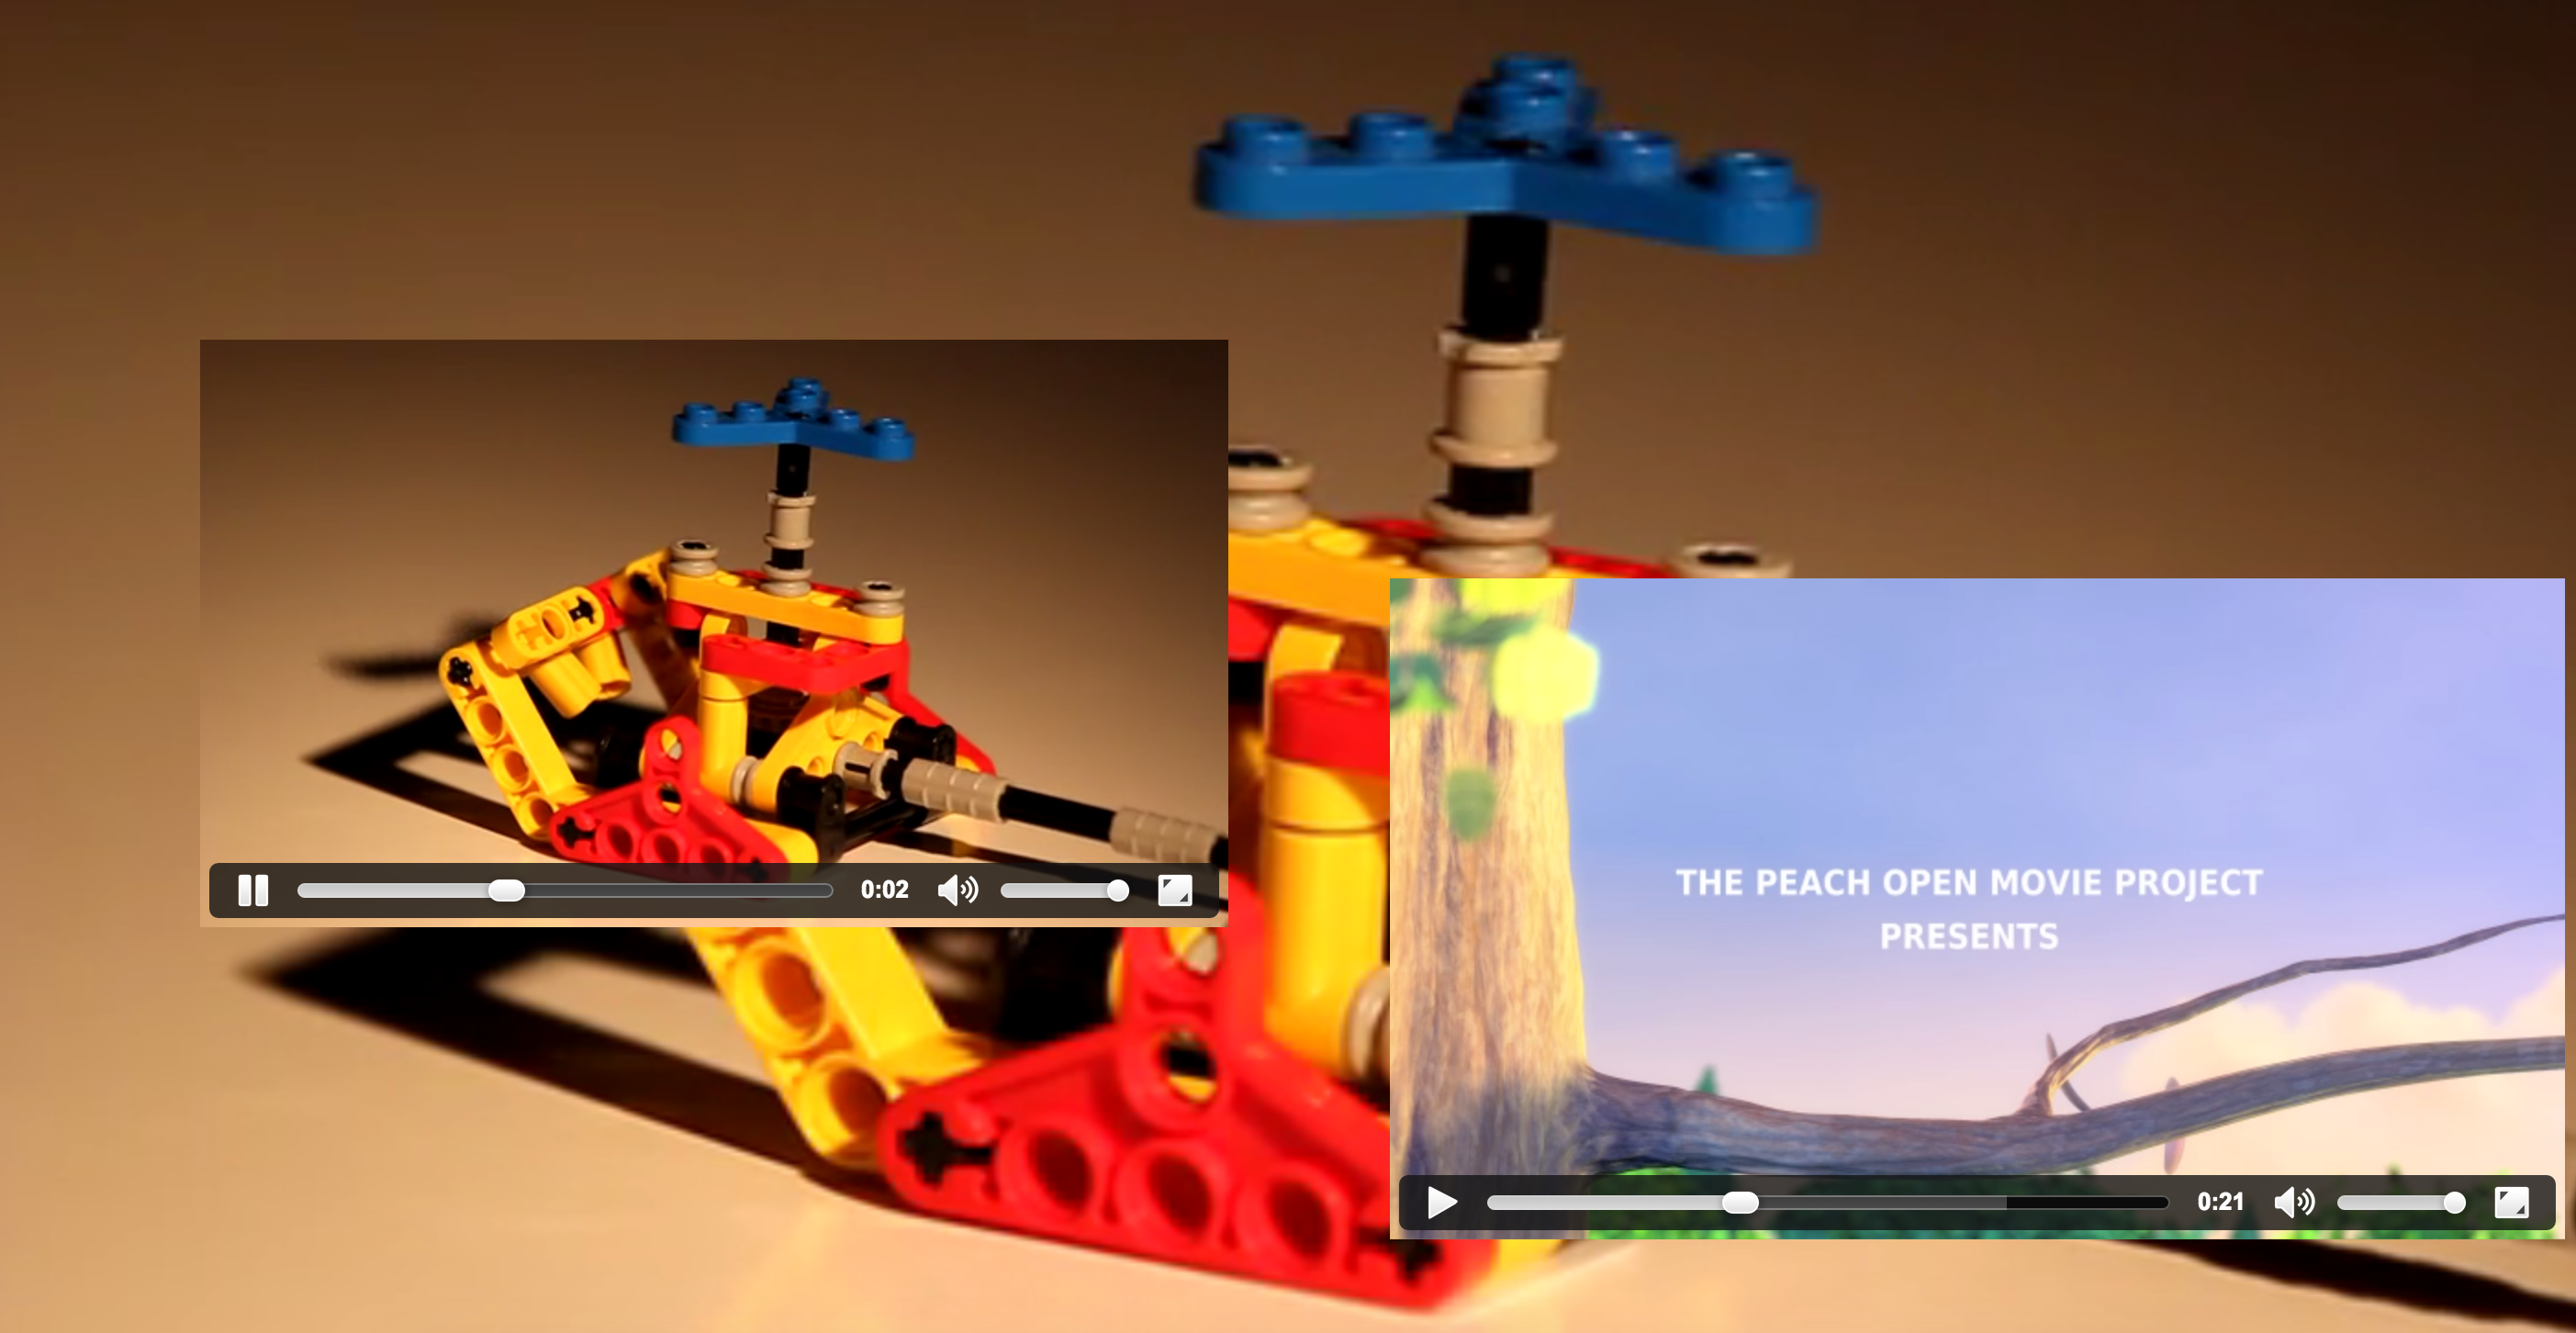
\includegraphics[height=176px, width=300px]{images/canvas2.png}\\
Abbilden eines Videos auf einem Canvas Objekt. 
\subsection{Drag-Drop}
\textbf{testcases - drag-drop - index.html} \\
Der Drag and Drop Testcase dient als Grundlage für die spätere Timeline.\\
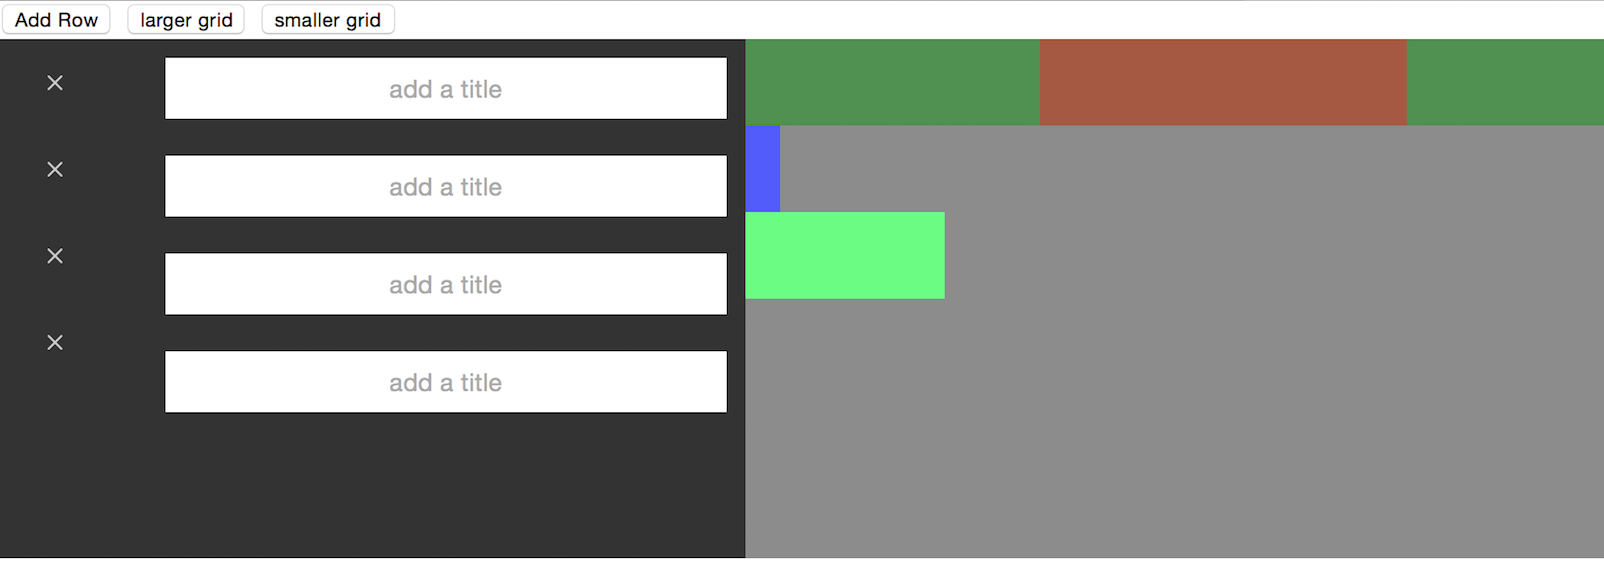
\includegraphics[height=176px, width=300px]{images/draganddrop.png}\\
Aus diesem Testcase wurde das Modul Video Timeline abgeleitet.\\
Es ist möglich neue Zeilen hinzu zu fügen und bestehende Leisten zu löschen.\\
Zudem kann man die hier farbigen Objekte, die spätere Videos darstellen sollen, innerhalb der leisten verschieben. Die Schritte in denen Verschoben wird, sprich die Größe des Grids ist einstellbar, damit wir später Stufenlos skalieren können.\\
Die Videos können in neue Zeilen gezogen werden, allerdings ist es nicht möglich, dass sich Videos überschneiden. 
\subsection{Video Export}
\textbf{testcases - export\_videos - index.html} \\
Dieser Test befasst sich mit der Möglichkeit Videos aus dem Browser zu exportieren. 
\subsection{Format Test}
\textbf{testcases - format-test - index.html} \\
\newpage
\subsection{Video Controls}
\textbf{testcases - video-controls - index.html} \\
Der Testcase Video Controls sollte die später benötigten Funktionen zum kontrollieren des Videos über JavaScript simulieren.\\ Folgende Funktionen wurden geschrieben und getestet : \\
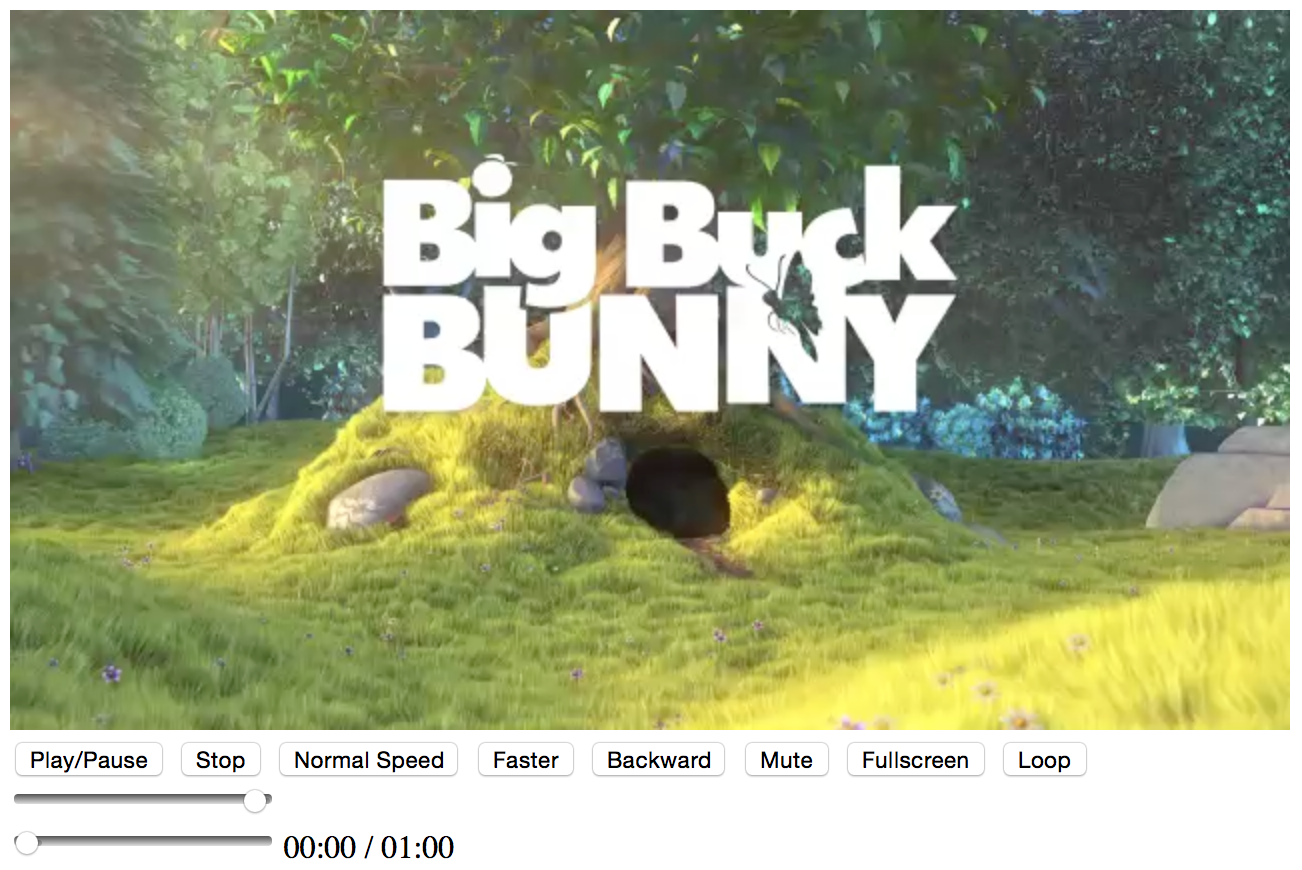
\includegraphics[height=176px, width=300px]{images/videocontrols.png}\\
\begin{itemize}
	\item Button
	\begin{itemize}
		\item Play/Pause
		\item Stop
		\item Faster / Normal Speed
		\item Backward
		\item Mute
		\item Fullscreen
		\item Loop
	\end{itemize}
	\item Slides
	\begin{itemize}
		\item Volume
		\item Current Time
	\end{itemize}
	\item Timeupdate
	\begin{itemize}
		\item Display Current Time
		\item Display Duration Time
	\end{itemize}
\end{itemize}
Das Crossbrowser Testing hat ergeben, dass einige Funktionen noch einmal überarbeitet werden müssen.\\
Aus diesem Testcase wurde das Modul Video Controls abgeleitet. 
\newpage
\section{Module}
\subsection{Video Item}
\textbf{testcases - module\_video\_item - index.html} \\
\textbf{videochop - js - modules - videoItem.js} \\
Jedes vom Nutzer in den Browser gezogene Video wird duch ein VideoItem repräsentiert. Es speichert alle relevanten Daten. Die Daten werden beim in den Browser ziehen vom Modul VideoItemLoader ausgelesen und in ein neues VideoItem geschrieben.\\
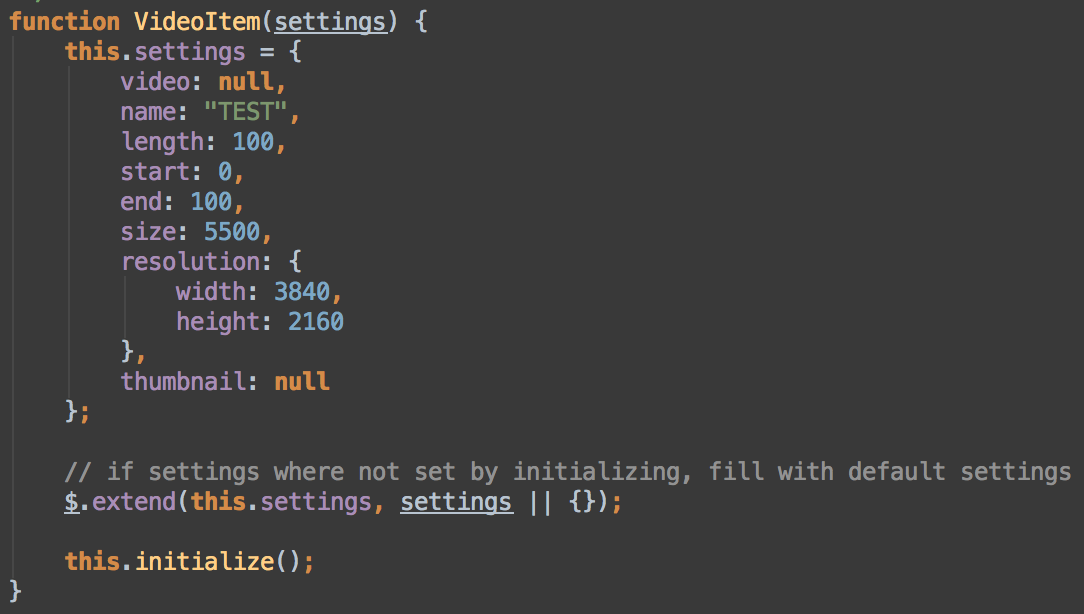
\includegraphics[height=176px, width=375px]{images/videoitem.png}\\
Das Videoitem bekommt die Eigenschaften Video-URL, Name, Länge, Startpunkt, Endpunkt, Größe, Auflösung und Thumbnail übergeben oder es werden die Default-Settings gesetzt.
In der Funktion getMarkUp() werden die HTML-Felder in der index.html dann mit den Werten des VideoItems befüllt, um es in der VideoItemList entsprechend anzuzeigen. \\
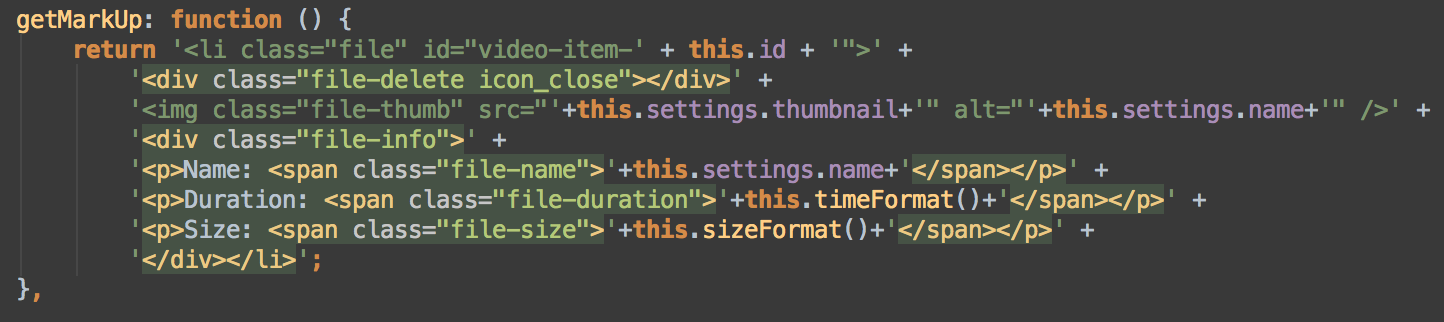
\includegraphics[height=120px, width=375px]{images/videoitem2.png}\\
Die Größe und die Länge des Videos werden formatiert in den Funktionen timeFormat() und sizeFormat().

\subsection{Video Item Loader}
\textbf{testcases - module\_video\_item\_loader - index.html} \\
\textbf{videochop - js - modules - videoItemLoader.js} \\
Mit diesem Modul wird nach dem Drag and Drop eines Videos vom Desktop in den Browser hinein ein neues VideoItem erstellt und zurückgegeben.\\
Es gibt die Attribute data, extension, name, prettySize, size und type welche zunächst auf Default-Werte gesetzt sind.
Wird ein neuer VideoItemLoader instanziiert, muss die Funktion add() aufgerufen werden, welche aus dem übergebenen Video eine Video-URL erzeugt. In der Funktion wird dann die Funktion loadMetaData aufgerufen und bekommt diese URL übergeben. In der Funktion wird ein Video-HTML-Element erzeugt und die URL wird diesem hinzugefügt. Anschließend wird ein neues VideoItem erzeugt und zurückgegeben, welchem die Eigenschaften des aktuellen Videos übergeben werden.
\subsection{Video List}
\textbf{testcases - module\_video\_list - index.html} \\
\textbf{videochop - js - modules - videoList.js} \\
Das VideoList Modul stellt den Container für die VideoItems zur Verfügung.\\
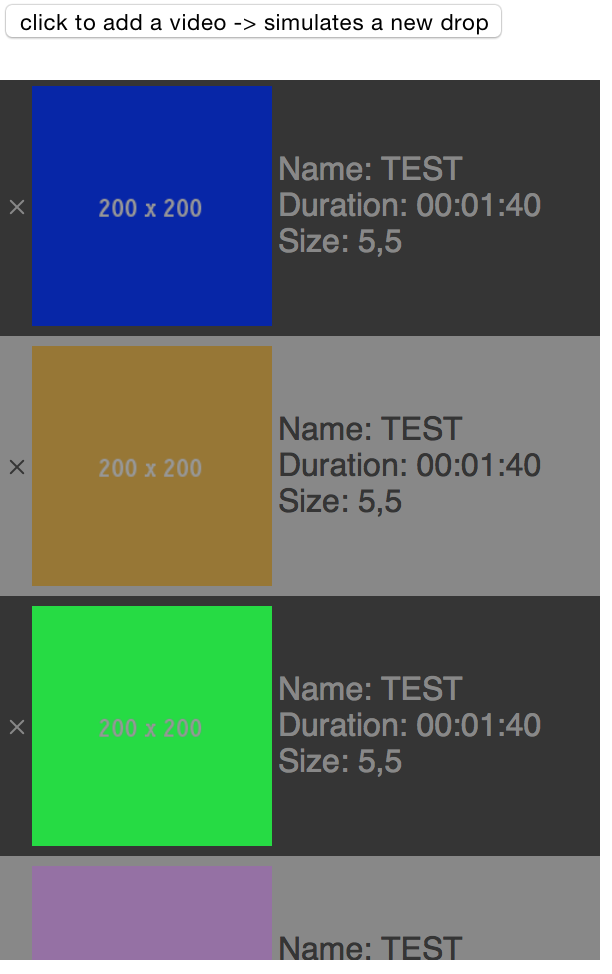
\includegraphics[height=300px, width=200px]{images/videolist.png}\\
\subsection{Video Preview}
Dieses Modul wurde noch nicht programmiert.\\
Stellt den Container für die Video Preview zur Verfügung.
\subsection{Video Controls}
Dieses Modul wurde noch nicht programmiert.\\
Stellt alle Funktionen zum kontrollieren der Videos zur Verfügung.
\subsection{Video Timeline}
Dieses Modul wurde noch nicht programmiert.\\
Das Video Timeline Modul stellt sämtliche Funktionen für die spätere Video Timeline zur Verfügung. 
\newpage
\section{Zeitaufwand}
\begin{tabular}{|c|c|c|}\hline
	\textbf{Aufgabe} & \textbf{Zeitaufwand} \\ \hline
	
	Projektkonzept & Zeitaufwand \\ \hline
	
	Einrichten Entwicklungsumgebung & Zeitaufwand \\ \hline
	
	Installation \& Konfiguration IDE & Zeitaufwand \\ \hline
	
	HTML-Struktur & Zeitaufwand \\ \hline
	
	JS-Module Template & Zeitaufwand \\ \hline
	
	Coding Conventions & Zeitaufwand \\ \hline
	
	Test-Case: Canvas & Zeitaufwand \\ \hline
	
	Mockup & Zeitaufwand \\ \hline
	
	Test-Case: Drag\&Drop & Zeitaufwand \\ \hline
	
	Test-Case: Video-Formate & Zeitaufwand \\ \hline
	
	Test-Case: Video Controls & Zeitaufwand \\ \hline
		
	Wiki: Lizenz prüfen & Zeitaufwand \\ \hline
	
	Logo & Zeitaufwand \\ \hline

	Mockup zu Layout & Zeitaufwand \\ \hline
	
	Test-Case: Video Controls Part II & Zeitaufwand \\ \hline
	
	Content: Impressum & Zeitaufwand \\ \hline
	
	HTML-Gerüst bauen & Zeitaufwand \\ \hline
	
	Test-Case: Drag\&Drop Part II & Zeitaufwand \\ \hline
	
	Video Controls: Cross Browser Test & Zeitaufwand \\ \hline
	
	Dokumentation: IDE & Zeitaufwand \\ \hline
	
	Test-Case: Drag\&Drop Part III & Zeitaufwand \\ \hline
	
	Module: VideoItem & Zeitaufwand \\ \hline
	
	Module: VideoList & Zeitaufwand \\ \hline
	
	Test-Case: Export Videos & Zeitaufwand \\ \hline
	
	Test-Case: Video-Converter & Zeitaufwand \\ \hline
	
	Module: VideoItemLoader & Zeitaufwand \\ \hline
	
	Präsentation des Projektstandes & Zeitaufwand \\ \hline
	
	Projektbeschreibung & Zeitaufwand \\ \hline
	
	HTML-Gerüst: Timeline & Zeitaufwand \\ \hline
	
	Test-Case: Video Part III & Zeitaufwand \\ \hline
	
	Test-Case: Canvas Part II & Zeitaufwand \\ \hline
	
	Module: Video Preview & Zeitaufwand \\ \hline
	
	FFMPEG & Zeitaufwand \\ \hline
 \end{tabular}
\newpage
\section{Quellen}
\end{document}